\documentclass{article}
\usepackage{amsmath}
\usepackage{amsfonts}
\usepackage{amssymb}
\usepackage{ctex}
\usepackage{graphicx}
\usepackage{float}
\usepackage{geometry}
\geometry{a4paper,scale=0.8}
\author{胡喜平\quad 李廷龙}
\title{量子计算的原理、发展、实现}
\begin{document}
\maketitle
\section{引言}
\label{sec:label}
量子计算(Quantum computing)最早于1969年提出,是指使用量子逻辑进行通用计算。与传统计算机不同,量子计算使用量子比特(quantum qubit)进行数据的存储与操作,使用量子算法进行数据操作。
\newline
从牛顿力学到相对论力学再到量子力学,力学在不断地发展。量子力学指出微观粒子的低速运动不遵从牛顿力学定律,而是满足薛定谔方程,呈现出特有的波粒二象性。其实要想对量子信息和量子计算进行深入的研究,也就是把量子力学原理应用于通信和计算机领域。
\newline
对计算机性能,也就是计算速度的不断要求,促使了计算机行业的不断发展,从每秒几千次运算,到几亿次运算。但是人们对运算速度的需求远不止如此,知道1982年,物理学家费曼第一次提出量子计算机,但是最开始只是停留在理论阶段,由于量子态的不确定性原理并且容易收到干扰,在运算额测量时很容易出错,一直到1994年计算机学家Shor才真正证明量子计算机的可行性 。但是,量子计算机与传统计算机相比在一些特定的问题求解方面有独特的优势。例如,在使用计算机模拟量子现象时,使用传统计算机模拟计算时,庞大的希尔伯特空间导致运算时间相当长,使用量子体系计算机能大大缩短计算时间。在质因数分解时,量子计算机的计算速度远高于传统计算机。这主要是因为量子计算机独特的构造。量子比特可以同时表示多种状态,而传统计算机里半导体只能记录0和1两种状态。同时,量子计算机对破解RSA加密算法等密码学领域有重大的意义,因此变成了热门的话题。

\section{量子计算的基本原理}
\label{sec:label}

\subsection{量子比特模型的建立}
\label{subsec:label}
传统的半导体计算机中比特只有两种状态,即0和1.量子比特不同与半导体比特的特殊之处在于量子比特时刻处于0和1的叠加态中。关于0和1的定义可以有多种方式,例如我们可以定义电子自旋向上为1,那么电子自旋向下就是0.因为叠加态的缘故,量子比特的数值可以在0和1之间任意取值。即
\begin{equation}
  \label{}
\vert \psi \rangle = \alpha \vert 0 \rangle + \beta \vert 1 \rangle
\end{equation}
其中$\alpha$和$\beta$是复数,且它们的模长平方和是1,量子比特在0状态和1状态的概率分别为$|\alpha|^{2}$和$|\beta|^{2}$
为了方便,我们用一个单位向量表示量子比特的状态
\begin{equation}
  \label{}
|\psi \rangle = \left(\begin{matrix}
    \alpha\\
    \beta
  \end{matrix}\right)
\end{equation}
则逻辑运算时的NOT门表示为
\begin{equation}
  \label{}
  X = \left(
    \begin{matrix}
      0 & 1\\
      1 & 0
    \end{matrix}
    \right)
\end{equation}
因为
\begin{equation}
  \label{}
X\left( \begin{matrix}
    \alpha\\
    \beta
  \end{matrix}\right)
=\left(\begin{matrix}
  \beta\\
  \alpha
\end{matrix}\right)
\end{equation}
即量子比特状态向量左乘$X$后反转.另一个量子计算时使用的逻辑门称为Hadamard门,它可以根据系数分解量子态,定义为:
\begin{equation}
  \label{}
H(\alpha | 0 \rangle + \beta | 1 \rangle ) = \frac{\alpha+\beta}{\sqrt{2}} | 0 \rangle + \frac{\alpha - \beta}{\sqrt{2}} | 1 \rangle
\end{equation}
用矩阵来表示为
\begin{equation}
  \label{}
  H=\frac{\sqrt{2}}{2}\left[
  \begin{matrix}
    1 & 1\\
    1 & -1
  \end{matrix}\right]
\end{equation}
同NOT门一样,连续使用两次Hadamard门后量子回到原先的状态。
\begin{figure}[H]
  \centering
  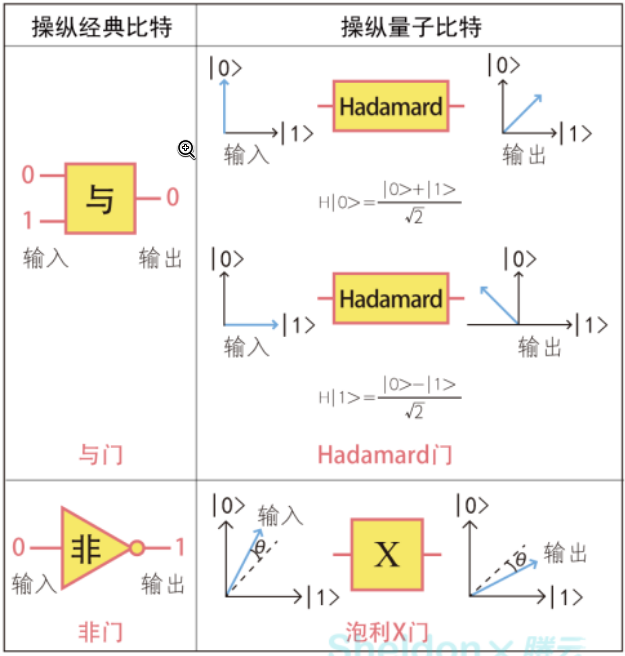
\includegraphics[width=0.6\linewidth]{figures/操控一个量子比特的逻辑门}
  \caption{操控一个量子比特的逻辑门}
\end{figure}
以上都是对于一个量子比特的逻辑门,对于用来条件判断的两个量子的逻辑门,在量子计算中由多输入多输出的受控NOT门实现。当第一个输入的量子比特是0时,对保持第二个输入比特不变。当第一个输入的量子比特是1时,则以NOT门作用于第二个比特。即:
\begin{equation}
  \label{}
CNOT(\alpha | 00 \rangle + \beta | 01 \rangle + \gamma | 10 \rangle + \theta | 11) = \alpha | 00 \rangle + \beta | 01 \rangle + \gamma | 11 \rangle + \theta | 10 \rangle
\end{equation}




\subsection{运用量子比特进行量子计算的原理}
\label{subsec:label}
经典计算机的计算大致分为三个过程,即输入数据,使用若干量子门对数据进行逻辑运算,输出数据。量子计算和经典计算机计算过程大致相同,输入量子比特,用量子门对量子比特进行操作,观测操作后的量子比特获取结果。主要的不同就是量子有叠加态,即一个量子比特可以表示0,同时也可以表示1,而在经典计算机中一个比特只能同时表示0或1中的一种情况。量子的叠加态在最后观察时才会坍塌到一种0或1的确定状态。因为量子的叠加特性,量子计算可以并行。上述叠加状态的一次演化相当完成了2个数据的并行处理,这就是量子计算机超并行计算的原理。两个量子比特可以一次进行4次运算,n个量子比特可以一次进行$2^{n}$次并行运算,而经典计算机一次只能进行一次计算。因此,量子计算在核爆模拟、密码破译、材料和微纳制造等领域具有突出优势,是新概念高性能计算领域公认的发展趋势。但是,由于量子比特本身及其不稳定,极容易和周围环境发成纠缠,微小的环境噪声都能对量子比特产生影响,导致计算错误。而且量子比特的数量越多,计算的错误率也就随之升高。在实际应用中需要一些手段来进行纠错。

\subsection{量子计算的物理实现方法}
\label{subsec:label}
以D-wave量子计算机为例,它主要是用约瑟夫森效应(Josephson effect)来构造量子比特进行计算。约瑟夫森效应是宏观量子效应的一种体现,当把两个超导体置于绝缘体的两侧时,由于量子隧穿效应,会产生一种超电流流过绝缘体,这种电流的产生不需要电压。中间的绝缘体称作约瑟夫森结。

\begin{figure}[htbp]
\centering
\begin{minipage}[t]{0.48\textwidth}
\centering
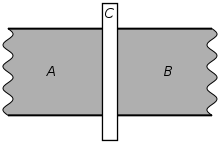
\includegraphics[width=0.4\linewidth]{figures/约瑟夫森结}
\caption{约瑟夫森结}
\end{minipage}
\begin{minipage}[t]{0.48\textwidth}
\centering
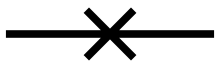
\includegraphics[width=0.4\linewidth]{figures/约瑟夫森结的电路符号}
\caption{约瑟夫森结的电路符号}
\end{minipage}
\end{figure}

约瑟夫森结中的超电流可能是正向,也可能是反向,且概率相等。因此可以作为量子比特来存储数据。
\begin{figure}[H]
  \centering
  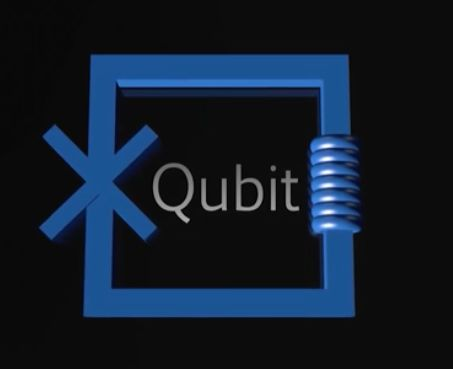
\includegraphics[width=0.5\linewidth]{figures/D-wave一个量子比特组成}
  \caption{D-wave一个量子比特组成}
\end{figure}
D-wave量子计算机的一个量子比特由一个环组成,在这个环里电流可能顺时针流,可能逆时针流。同时,可以通过施加垂直于线框的磁场来改变里面的电流,达成对量子比特的控制。
\begin{figure}[H]
  \centering
  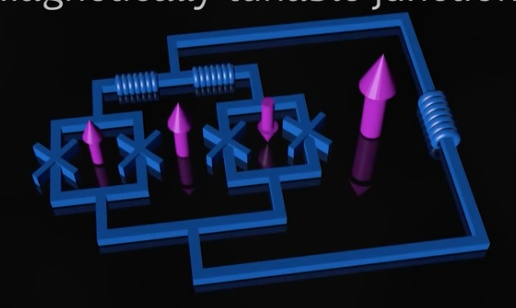
\includegraphics[width=0.7\linewidth]{figures/最终量子比特设计}
  \caption{最终量子比特设计}
\end{figure}
当然,这只是初级的设计。为了更精准地对量子比特进行控制,后续加入了势井和更多的磁场。除了使用超导约瑟夫森结实现量子运算的方案以外,还有应用离子阱、中性原子的能级、光的偏振等实现量子比特的方案,各中实现方案各有优劣。
\section{量子计算的现状}
现在的量子计算除逻辑比特是量子比特外,计算模型还是借用经典的图灵机模型,整个量子计算过程可分解为两种基本量子逻辑门的大量组合。这种模型的好处是通用性好,量子计算机能解决的问题原则上都可用此模型实现,缺点是结构复杂,需要大量的逻辑门操作,未来 20-30 年甚至更长时间都难以实现。但不是所有问题的解决量子计算机都优于经典计算机,量子计算机没必要完全取代经典计算机,只要能解决部分经典计算机不能或难以解 决的问题就很有意义。针对特殊问题的量子计算(称之为专用量子计算),可以通过设计特殊的计算模型和特殊的量子算法,避免大量的逻辑门操作,大大简化计算的复杂性,有望在未来10年内实现。加拿大D-Wave公司就是采取所谓的绝热量子计算模型实现退火算法。另外,由于量子系统有未知量子态信息不可复制、量子态信息的保存 时间不能像经典态一样可以很长、量子态可以是多个态的叠加等特点,量子计算机可能需要不同于冯·诺依曼体系结构的新体系结构。因此专用量子计算及其相关的计算模型和量子计算机体系结构的研究是未来量子计算研究的重点之一,有可能对未来计算机科学产生重大影响。
\newline
目前典型的量子算法是搜索算法和大数质因子分解算法。但这些算法都是以一些基本运算为基础,而这些基本运算的量子算法还没有提出。另外,最近发现一些能实现的量子演化过程能被应用于某些复杂问题的求解。 如2013年Science杂志连续发表2篇文章报道通过玻色 采样的物理过程能实现矩阵积和的求解(该问题 是经典计算机的NP难解问题。利用已实现的量子过程来模拟某些复杂问题的求解及其相应算法可能使某些难解决的问题能很快得到解决,有望10年左右能实现一些特殊问题的专用量子计算。因此我们认为,量子算法的研究重点是基本运算的量子算法、用已实现的量子过程对复杂问题的模拟及其相应算法的研究。量子计算是量子物理与计算机科学交汇而生的一门新兴学科。它的出现实质上是量 子物理学向物质 、能量和信息这三大领地的最后一块-信息领域的进军 。尽管我们不应奢望量子计算机能完全取代经典计算机, 但量子计算的某些令人惊诧的本领着实让人着迷 和刮目相看。尽管如此, 量子计算发展至今, 我们所完成的实验都只是少数几个量子比特 的量子计算演示性实验,量子计算的威力还远远未能显现出来 。我们今天仍不能肯定真正的量子计算机将是什么样子、有哪些功能 。因此, 我们既可以乐观地认为量子计算能最终给我们带来一场新的技术革命, 也可以保守地认为量子计算的研究最多只能带给我们一些副产品而并非量子计算机本身。但不管怎样 ,对量子计算的研究已经使我们重新认真思考了诸如纠缠、消相干等原来并未完全弄清楚的问题, 它也带给我们新的思维方式。更重要的是它向我们提出了新的问题。量子计算所包含的迷人的思想将激励人们更深入地了解经典世界和量子世界的关系 ,发掘自然界更深层次的规律和人类自身的潜力 。
\newline
我国从事量子计算实验研究的主要单位是中国科技大学、清华大学、国防科技大学、南京大学 和中国科学院武汉物理数学研究所等, 各单位在 这方面的研究整体上都处于起步阶段。 中国科技大学主要从事光子、量子点和核自旋的量子计算 研究。2013 年,他们用光量子技术展示了线性方程组求解;2014年基于光量子系统完成了Landau-Zener 动力学演化过程的量子模拟原理演示;2012年,利用4量子比特完成了143 的质因子分解;2014 年,采用压缩量子模拟技术,利用5量子比特系统模拟了32个粒子组成的自旋链。清华大学主要研究离子和核自旋的量子计算,国防科技大学和中国科学院武汉物理数学所主要研究 离子系统的量子计算,
南京大学主要研究超导的量子计算。这些单位都建成了相应的实验平台,具 备了开展高水平研究的条件。

\begin{thebibliography}{99}  
\bibitem{ref1}量子计算的物理实现, 薛 飞, 杜江峰, 周先意, 韩荣典, (中国科学技术大学近代物理系 合肥)
\bibitem{ref2}Josephson effect, https://en.wikipedia.org/wiki/Josephson\_effect
\bibitem{ref3}D-Wave Systems, https://en.wikipedia.org/wiki/D-Wave\_Systems
\bibitem{ref4}量子计算机的工作原理如何解释, https://www.zhihu.com/question/30545465
\bibitem{ref5}10分钟看懂量子比特、量子计算和量子算法 https://zhuanlan.zhihu.com/p/27387032
\bibitem{ref6}Quantum computation using quantum dots, Xin Wang, City University of Hong Kong
\end{thebibliography}

\end{document}